\section{Mode 1 - Writting letters}
The first mode allows user to select and write proper letter. In english alphabet there are 26 letters, so to be able to use all of them a lot of gestures had to be specified and implemented. Our aim was to do this as simple as possible, because too complicated set of movements and signs could have not been user-friendly and straightforward. The scheme was shown in the Figure \ref{fig:letters}.

\begin{figure}[H]
	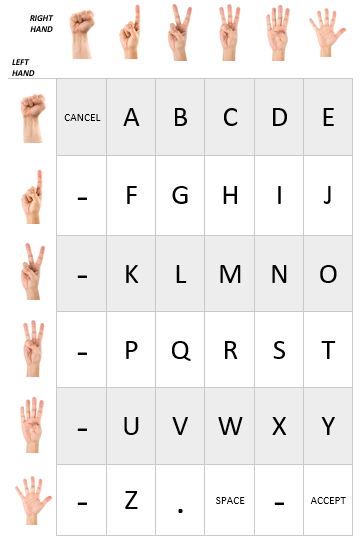
\includegraphics{static_gestures}
	\centering
	\caption{Letter selection - set of gestures}
	\label{fig:letters}
\end{figure}

Every letter and command had its own and unique command. \textbf{By counting number of extended fingers in either hands differentation was done}. It was very clear and easy to learn set of gestures. For instance, when in the left hand only one finger was extended and in the same moment the right hand was fully open then it meant that letter "J" should have been drawn. The system worked well only when leap was detecting both hands.\\

Sometimes wrong letter was selected and to avoid wrong comunication with the robot two additional gestures were added - command "Accept" to send proper letter to the robot and command "Cancel" to reset current letter and repeat selection. We wanted also to write full sentences. Thus we decided to implement gesture to draw dot and one more to make space between two words. It is easy to see in the Figure \ref{fig:letters} that there are 6 more possible gestures that were not used. That set of gestures can be easily extended. 